\documentclass[12pt, a4paper]{article}

\usepackage[utf8]{inputenc}
% Limit the page margin to only 1 inch.
\usepackage[margin=1in]{geometry}

%Imports biblatex package
\usepackage[
backend=biber,
style=alphabetic
]{biblatex}
\addbibresource{../../algs4e.bib}

% Enables the `align' environment.
\usepackage{amsmath}
% Provides useful environments, such as:
% - \begin{proof} ...\end{proof}
\usepackage{amsthm}
\usepackage[most]{tcolorbox}

\newtheorem*{proposition}{Proposition}

% Enables using \mathbb{}, for example \mathbb{N} for the set of natural numbers.
\usepackage{amssymb}

% Allows using letters in enumerate list environment. Use, for example:
%\begin{enumerate}[label=(\alph*)]
% ...
%\end{enumerate}
\usepackage[inline]{enumitem}

% Enable importing external graphic files and provides useful commannds, like \graphicspath{}
\usepackage{graphicx}
% Images are located in a directory called images in the current directory.
\graphicspath{{./images/}}

% Make links look better by default.
% See: https://tex.stackexchange.com/questions/823/remove-ugly-borders-around-clickable-cross-references-and-hyperlinks
\usepackage[hidelinks]{hyperref}
\usepackage{xcolor}
\hypersetup{
	colorlinks,
	linkcolor={red!50!black},
	citecolor={blue!50!black},
	urlcolor={blue!80!black}
}


% Code Listings. Source:
% https://stackoverflow.com/questions/3175105/inserting-code-in-this-latex-document-with-indentation
\usepackage{listings}
\usepackage{color}

\definecolor{dkgreen}{rgb}{0,0.6,0}
\definecolor{gray}{rgb}{0.5,0.5,0.5}
\definecolor{mauve}{rgb}{0.58,0,0.82}

\lstset{frame=tb,
	language=Java,
	aboveskip=3mm,
	belowskip=3mm,
	showstringspaces=false,
	columns=flexible,
	basicstyle={\small\ttfamily},
	numbers=none,
	numberstyle=\tiny\color{gray},
	keywordstyle=\color{blue},
	commentstyle=\color{dkgreen},
	stringstyle=\color{mauve},
	breaklines=true,
	breakatwhitespace=true,
	tabsize=3
}

\newcommand{\prob}{\text{P}}
%\newcommand{\complement}{\mathsf{c}}

% Define an environment called "ex" (for Exercise) so that I can do: \begin{ex}{1.5}...\end{ex}
\newenvironment{ex}[2][Exercise]
{\par\medskip\noindent \textbf{#1 #2.}}
{\medskip}

% Define a solution environment, similar to ex (exercise) environment.
\newenvironment{sol}[1][Solution]
{\par\medskip\noindent \textbf{#1.} }
{\medskip}

\begin{document}
	\noindent Sergio E. Garcia Tapia \hfill
	
	\noindent \emph{Algorithms} by Sedgewick and Wayne (4th edition) \cite{sedgewick_wayne}\hfill
	
	\noindent December 1st, 2024\hfill 
	\section*{3.2: Binary Search Trees}
	\begin{ex}{1}
		Draw the BST that results when you insert the keys \texttt{E A S Y Q U E S T I O N},
		in that order (associating the value \texttt{i} with the \texttt{i}th key, as per the
		convention in the text) into an initially empty tree. How many compares are needed
		to build the tree?
	\end{ex}
	\begin{sol}
		The sequence of binary search trees is shown in Figure~\ref{fig:ex-01}. The boxes next
		two the root show the number of compares necessary to complete the insertion at
		that step. The sequence of compare counts is: 0, 1, 1, 2, 2, 3, 1, 2, 4, 3, 4, 5.
		Adding gives a total of 28 compares.
		\begin{figure}
			\centering
			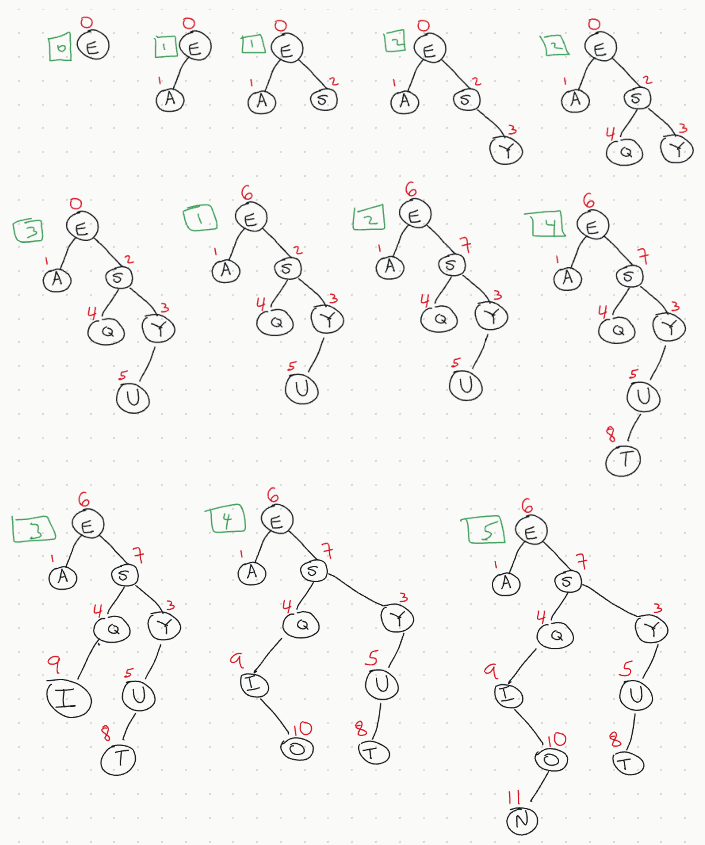
\includegraphics[width=0.7\textwidth]{exercise-01}
			\caption{Exercise 1: Sequence of trees formed when inserting the keys \texttt{E A S Y Q U E S T I O N}
			into a binary search tree.}
			\label{fig:ex-01}
		\end{figure}
	\end{sol}
	\begin{ex}{2}
		Inserting the keys in the order \texttt{A X C S E R H} into an initially empty BST
		gives a worst-case tree where every node has one null link, except one at the bottom,
		which has two null links. Give five other orderings of these keys that produce
		worst-case trees. 
	\end{ex}
	\begin{sol}
		We can insert them in the following ways:
		\begin{enumerate}[label=(\roman*)]
			\item \texttt{A X C S E R H} (given).
			\item \texttt{X S R H E C A}.
			\item \texttt{A C E H R S X}.
			\item \texttt{X A S C R E H}.
			\item \texttt{X A S R H E C}.
			\item \texttt{A X C E H R S}.
		\end{enumerate}
		See Figure~\ref{fig:ex-02}.
		\begin{figure}
			\centering
			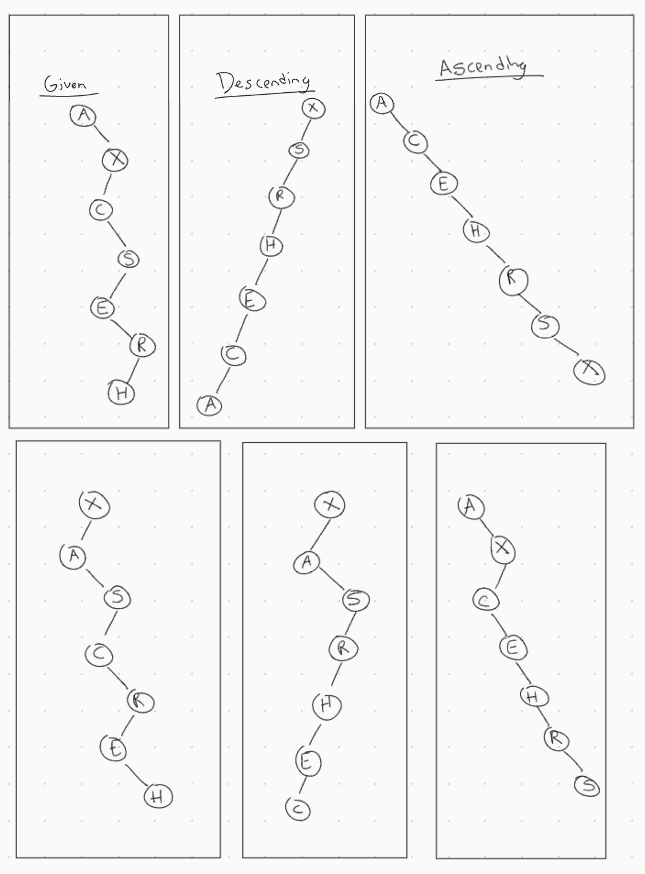
\includegraphics[width=0.7\textwidth]{exercise-02}
			\caption{Exercise 2: Worst-case binary search trees created by inserting the
			keys \texttt{A X C S E R H} into an initially empty tree in a particular order}
			\label{fig:ex-02}
		\end{figure}
	\end{sol}
	\begin{ex}{3}
		Give five orderings of the keys \texttt{A X C S E R H} that, when inserted into an
		initially empty BST, produce the \emph{best-case} tree.
	\end{ex}
	\begin{sol}
		\begin{enumerate}[label=(\roman*)]
			\item \texttt{H C S A E R X}.
			\item \texttt{H S C A E R X}.
			\item \texttt{H S C E A X R}.
			\item \texttt{H S R X C A E}.
			\item \texttt{H S X R C A E}.
		\end{enumerate}
		These all result in the same tree, depicted in Figure~\ref{fig:ex-03}.
		\begin{figure}
			\centering
			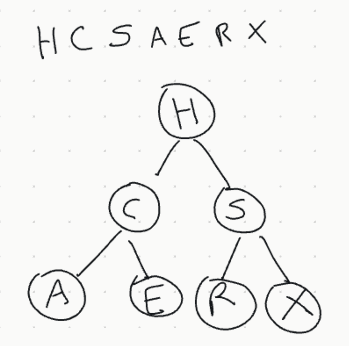
\includegraphics[width=0.3\textwidth]{exercise-03}
			\caption{Exercise 3: Best-case binary search trees created by inserting the
				keys \texttt{A X C S E R H} into an initially empty tree in a particular order}
			\label{fig:ex-03}
		\end{figure}
	\end{sol}
	\begin{ex}{4}
		Suppose that a certain BST has keys that are integers between \texttt{1} and \texttt{10},
		and we search for \texttt{5}. Which sequence below \emph{cannot} be the sequence
		of keys examined?
		\begin{enumerate}[label=(\alph*)]
			\item \texttt{10, 9, 8, 7, 6, 5}
			\item \texttt{4, 10, 8, 6, 5}
			\item \texttt{1, 10, 2, 9, 3, 8, 4, 7, 6, 5}
			\item \texttt{2, 7, 3, 8, 4, 5}
			\item \texttt{1, 2, 10, 4, 8, 5}
		\end{enumerate}
	\end{ex}
	\begin{sol}
		\begin{enumerate}[label=(\alph*)]
			\item This is a valid sequence. For example, this could be a tree where the
			keys were inserted in descending order.
			\item This is a valid sequence.
			\item This is a valid sequence.
			\item This sequence cannot happen. The sequence of compares suggests the following:
			\begin{enumerate}[label=(\roman*)]
				\item 2 is the root, and 5 is larger, so we go right.
				\item 5 is smaller than 7, so we go left.
				\item 5 is smaller than 3, so we go right.
				\item 5 is compared against 8.
			\end{enumerate}
			This last step is impossible because since 8 is larger than 7, but it
			appears on the subtree rooted at its left child, consisting of smaller
			keys,  a contradiction.
			\item This is a valid sequence.
		\end{enumerate}
	\end{sol}
	\pagebreak
	\printbibliography
\end{document}